\documentclass[a4paper,11pt]{article}

\usepackage{graphicx, url}

%--Title---------
\title{Software Evolution - Assignment 2 : Architecture Reconstruction}
\author{Stef van Schuylenburg (0744314) \& Jules Wulms (0747580)}
\date{\today}
%----------------

\begin{document}

	\maketitle

	\section{Introduction}
		In this assignment we reconstruct the architecture of a Java program. To show the architecture we create a UML class diagram containing the classes, fields, methods and relations between the classes. This diagram is created by first extracting the information from the java program using a program written in Rascal\cite{rascal}.	Then we use this information to construct the classes, the fields and methods of the classes and the relations between the classes. In order to find all the relations we also use an Object Flow Graph. This graph allows us to calculate where objects are used, and thus what class of objects are used by a container or other class, of which we cannot directly specify the type. In the end we visualize all our extracted information into a UML class diagram. For the visualization we use Rascal to generate a DOT-file of the class diagram, this DOT-file is then read by GraphViz\cite{graphviz} to draw a pdf-image containing the diagram. \\

		To test this tool chain, wel reconstruct the architecture of a Java project named \textit(eLib). eLib is used in a book by F. Tonella and A. Potrich \cite{tonella}, and we check our own reconstruction by comparing with the example in the book. When the tool chain is able to reconstruct eLib's architecture, we can use it on a bigger project. We look into the evolution of a Java project named CyberNeko HTML Parser. It is a much bigger project and we will reconstruct the architecture of a 2007 and a 2010 version. This way we can see how the project has evolved. \\

		The report has the following structure: In Section 2 we elaborate on the input and output of our tool chain. Section 3 is about the design and usage of the tool chain. Section 4 is about the application of the tool chain, to eLib and to the different versions of CyberNeko HTML. In Section 5 we discuss the advantages en disadvantages of our tool chain. The report ends with conclusions we can draw from developing a reconstruction tool and doing a case study about the evolution of an architecture.
	
	\section{Input and Output}
		The general approach of our tool chain is that we take a Java project as input and give a visualized UML class diagram of this Java project as output. In this section we look at the input and output in more detail to indicate what our tool chain exactly accepts and what it returns.
		
		\subsection{Input}
			We support the following features of the Java language:
			\begin{itemize}
				\item non-nested Classes: Classes are the main components of the UML Class diagram so, should have to be included to make the class diagrams.
				\item methods: The methods show the main functionality of a class and are used to find dependencies between classes.
				\item fields: The fields are used to create the associations and are used in the class description.
				\item generics: Generics are used to define the structure of a class or method, so we also have to include those. Since generics are really broad in Java, we choose to support the following parts: Generic classes and variables, which are things like \texttt{ArrayList<Integer>}. Furthermore we support methods that use generics, like \texttt{void <M> doSomething()}.
				\item inner classes: It is possible that classes depend on innner classes of other classes. So without the inner classes we are not able to create a complete class diagram.
				\item visibility: Visibility, to represents the scope of functions and thus also the functionality of class.
				\item static: Static fields and methods are not attributes of instances of a class, but can be used by all instances. So we have to show what is static, such that it is clear that all instances may depend on each other (as they use the same functions).
				\item extends and implements relation: The extends and implements relations is used to create the generalization and realization relations of the class diagram. Those relations are very important for the architectural structure.
			\end{itemize}
		
			We do not use the following features of the Java language:
			\begin{itemize}
				\item annotations: In Java annotations can be defined by any library or by the program itself, so supporting annotations would require an additional system to keep track of all the annotations. To make things not to complex, the annotations are not used in our tool chain.
				\item a number of modifiers: A number of modifiers like synchronized, volatile, native are not used in our system. We did not include those, because the modifiers are not often used and they do not add usefull information for the architecture; most of thesecmodifiers are about the implementation of the method or usage of a field.
			\end{itemize}
		
		\subsection{Output}
			The output of our tool chain is the class diagram. We did include the following features of a class diagram:
			\begin{itemize}
				\item classes: The basic component of the class diagram, included to show what classes are part of the program.
				\item fields and methods: Those are included to show the functionality of a class. We also decided to include the private fields and methods, because they can be a reason for some associations and dependencies.
				\item associations, dependencies, generalization and realization: Used to show the structure of our system. We use the standard UML notations, assosiations are arrows, dependencies are dashed arrows, generalizations are arrows with open heads, and realizations are dashed arrows with open heads. 
				\item ``named associations'': Our associations are named in such a way that the name of the field is also used for the association. This makes it clears what the association represents and makes it also possible to have multiple association from one class going to the same class.
				\item inner classes: Inner classes look exactly like non-nested classes in the UML diagram. However there is an arrow with a dot at the end, connecting the inner class to the class it is nested in. The dot-arrow will mimic the open-dot-with-plus-inside-arrow, which is often used for inner class relation.
			\end{itemize}
		
			The following features are not included in our output:
			\begin{itemize}
				\item two-directional associations: We did not include those, because we prefer to use two one-directional associations. The one-directional associations prevent the problem, where sometimes it is misunderstood whether the fieldname belongs to one class or to the other. Also the associations are still clear when we only use the one-directional associations. Also the names that are given to two-directional associations, to show the intent of the relation between two classes, are impossible to retrieve from the code. Guessing the names requires a whole algorithm on its own.
				\item multiplicity: We did not include the multiplicity, because we can only find $0..1$ and $0..*$, when we extract the multiplicity from a program. Only these two are found, because an association is either created from a collection ($0..*$) or a simple field($0..1$). We can easily find the multiplicity by looking at the type of the associated field, so adding the multiplicity would only make the diagram more complex. Since GraphViz automatically generates a class diagram, as if it is a graph, we cannot assure that everything will be nicely structured, and keeping things simple will make a diagram more readable. 
			\end{itemize}
		
	\section{The Tool Chain}
		For our tool chain we use two different programs to execute it: Rascal and GraphViz. The main part of our tool chain is our program written in Rascal, which outputs a DOT-file for GraphViz.
		
		\subsection{Rascal Program}
			We have divided our program in 3 components: \emph{Extraction}, \emph{OFG} and \emph{Visualize}, those components are Rascal modules and Extraction and Visualize can be used in isolation. OFG creates the Object Flow Diagram and is used in both Extraction (for the extraction of associations) and Visualize (to visualize the OFG). Besides these components we also have two other modules: \emph{DiagramLanguage} and \emph{Main}. DiagramLanguage defines the datatypes that are used to transfer the extracted data from Extraction to Visualize and Main is used to execute everything. \\
	
		\subsubsection{Extraction}
			The Extraction module has functions to extract all the information needed for a Diagram (as defined by the DiagramLanguage) from a Java project. This modules uses the Java-extraction libraries from Rascal (found in the modules \texttt{\url{lang::java::jdt::m3::AST}} and \texttt{\url{lang::java::jdt::m3::Core}} to extract the classes, fields, methods and a number of relations from the Java project and to construct the Diagram with it. It also uses the OFG module to find associations that can not be found using standard extraction of the Java project. The main method that is used to generate the Diagram using the Extraction module is called \texttt{onsDiagram(M3 m)}. The Diagram consists of all Classes (with Fields an Methods) and all Relations (from Class to Class, possibly linked to a Field). \\
		
			In Extraction we mostly use comprehensions to create sets of data we want to use. By iterating over these sets, we put all the data in datatypes defined in DiagramLanguage. However, we should be carefull when defining comprehensions, because each added set we iterate over will increase the running time multiplicative. So if we iterate over set $A$ we get $A$ iterations, and also iterating over $B$ gives $A*B$ iterations. This makes the Extraction modules a bit slow, especially when extracting relations between classes. We did not do many optimizations here, since the goals is to retrieve the architecture within a reasonable amount of time, not to write the most optimal retrieval program.
	
		\subsubsection{OFG}
			The OFG module is a module to create an Object Flow Graph and to get the relations from this Object Flow Graph which will represent associations in the output diagram. OFG uses the \emph{Rascal-OFG}\cite{rascal-ofg} code to create the Object Flow Graph. After creating the Object Flow Graph the module uses this graph to create the associations which are used by the Extraction module. \\

			The main method, which is used to find the relations from certain objects to others can be found at \texttt{cacl(Program prog, bool forward)}. What this function does is, it builds the OFG, which is done by \texttt{buildGraph(Program p)}, and then uses \texttt{prop(OFG g, rel[loc,loc] gen, rel[loc,loc] kill, bool back)} to propagate object through the graph. Both these functions are expansions of the code shown by Dr. Jurgen Vinju in his guest lecture at TU/e. The generate and kill sets used for forward and backward propagation are defined according to Chapters 2 and 3 in the book by Tonella and Potrich \cite{tonella}. 
	
		\subsubsection{Visualize}
			The Visualize module creates a string formatted in the DOT language which is used to render the diagram. This module takes a diagram as input and uses code generation to create a DOT-file. The DOT-file is intended to be used by GraphViz to create an image describing the diagram as a UML Class Diagram. The main method, which takes a diagram and creates the DOT-file for it is called \texttt{diagram2dot(Diagram diagram)}. An extra function, which we created to visualize the Object Flow Graph, generated by OFG, is \texttt{OFG2dot(Program prog)}. This also needs \emph{Rascal-OFG} to generate the Program for a Java project. The OFG itself will be constructed in \texttt{OFG2dot}. \\
	
			We decided to use those components and to decouple Extraction and Visualize, such that we can easily use a different kind of visualization or a different kind of extraction. It also allows us to work seperated on those components and to rarely have to change one component because the other has changed. It also makes testing easier. For example, we do not have to extract data from a Java project (which can take quite some time) in order to test the Visualize module. \\
	
			Instead of using the style we explained above, where another module (the Main module) uses the components to pass the return value of one to the other (like the pipe and filters style), we could also let Visualize depend on Extraction or vice versa. We decide to not do this, because this makes it easier to replace one of the components by something else. It is also easier work with a new language, if we could stay true to the modular way of programming we are used to. However, having two separated components, that each iterate over a lot of data have made the program a bit slower than it could have been, when output would be generated in the same iteration as the extraction.
	
		\subsection{GraphViz}
			To create an image of the diagram we use GraphViz. We use the DOT code generated by the Visualize module of our program. The GraphViz tools takes this DOT code as input and returns an image as output.
	
		\subsection{Usage of the Tool Chain}
			To use the Tool Chain we have created a Main module. This Main module contains a function called \texttt{run(loc project, loc file)}. Which creates DOT output for the eclipse program specified in \texttt{project}. (\texttt{project} is a Rascal location, so if you want to use for example the eclipse program eLib, then \texttt{project} would be \texttt{|project:///eLib|}.) After calling the run function, DOT output for the diagram will be saved in \texttt{file}. Now we need GraphViz to generate the image using \texttt{file}. \\
	
			Assuming that GraphViz is installed the image can be generated with the following command: ``\texttt{dot -Tps in.dot -o out.pdf}'' with \texttt{in.dot} being the location of the DOT-file and \texttt{out.dot} being the location, where you want to save the image of the class diagram.
	
	\section{Application of Tool Chain}
		The tool chain is developed for reconstructing architectures, so we applied it on some Java projects to see how it performs and to address the evolution of an existing Java project. In this section we will first compare the results of our own tool chain to the results shown in in the book by Tonella and Potrich \cite{tonella}, and after that look into the evolution of CyberNeko HTML Parser, by reconstructing the architecture of 2 versions of the project.
		
		\subsection{eLib}
			We started off  by using our tool chain on the \emph{eLib} project. We used eLib in the development process, as a means of checking what was good and which parts of the model needed changes/additions. \\

			Figure \ref{fig:elib1} shows the class diagram of eLib, with all the class-specific features and all relations between the classes. It has the expected structure, which makes us believe that all the information in extracted as it should. As you can see, the diagram is pretty clear, but being very critical, we can come up with some possible enhancements:
			
			\begin{itemize}
				\item Some relations are not as fully visible as others. If we look at the bottom side of Loan, we see that up to 4 arrows start/end in the same point, which could be done more clearly.
				\item The hierarchy and grouping of the classes is not clearly present in this visualization. An example of this is the specializations of Document and User are places above them in the class diagram, while the structure could be simpler when they were placed below as in the Tonella and Potrich book \cite{tonella}. Also the specializations of Document are split by relation arrows between Document and Library/Main.
			\end{itemize}
			
			\begin{figure}[h!]
				\centering
				\includegraphics[width=\textwidth]{eLib1}
				\caption{Reconstructed class diagram for eLib.}
				\label{fig:elib1}
			\end{figure}
			
			When this class diagram was fully working, we added some features to eLib, so that we could also test inner classes and generics. This led to the diagram in Figure \ref{fig:elib2}. We gave book generics of both of the supported types, and an inner class named Bladzijde. Regarding visualization, we see in this version that the overlapping arrows are separated at Loan, but the inner class and association relation of Book and Bladzijde are too close together. The hierarchy or grouping of certain classes is still the same, so if we would want to express that classes are in a group or of the same order so that they can be put together. \\

			\begin{figure}[h!]
				\centering
				\includegraphics[width=\textwidth]{eLib2}
				\caption{Reconstructed class diagram for edited version of eLib (with inner class and generics).}
				\label{fig:elib2}
			\end{figure}

			We also tried to visualize the OFG that is build in the extraction process. The whole OFG can be found in Figure \ref{fig:ofgelib} as appendix. We want to highlight some important parts of the OFG in Figures \ref{fig:users}, \ref{fig:docs} and \ref{fig:loans}. In Figure \ref{fig:users}, we see how the classes User and its specialization flow to the field in Library. Figure \ref{fig:docs} shows how the specializations of Document flow to Library. Document itself, for Library.documents, can only be found by backward propagation, which also goes through an iterator. This process is too big to show here. \\

			We want to point out that the outcome of flow propagation for specialized classes is ignored, when there is also flow for the general class. We see this for the specializations of both User and Document. Since they both flow the the respective fields of Library, we ignore the flow from the specialized classes, since it will only lead to redundant associations. \\

			The flow propagation of Loan, to the fields in User and Library can be seen in Figure \ref{fig:loans}. We see that up to a certain point the flow propagation is identical to both these fields. \\

			\begin{figure}[h!]
				\centering
				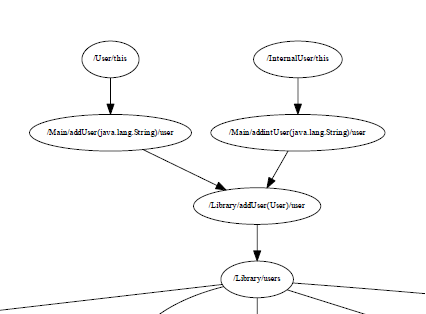
\includegraphics{users}
				\caption{Reconstructed class diagram for edited version of eLib (with inner class and generics).}
				\label{fig:users}
			\end{figure}

			\begin{figure}[h!]
				\centering
				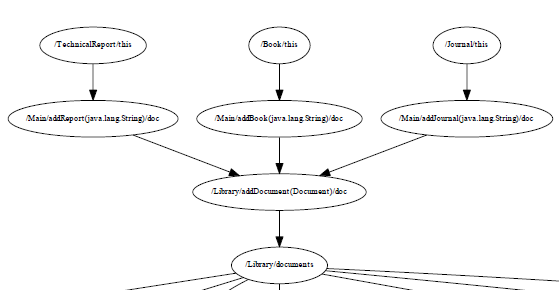
\includegraphics{documents}
				\caption{Reconstructed class diagram for edited version of eLib (with inner class and generics).}
				\label{fig:docs}
			\end{figure}

			\begin{figure}[h!]
				\centering
				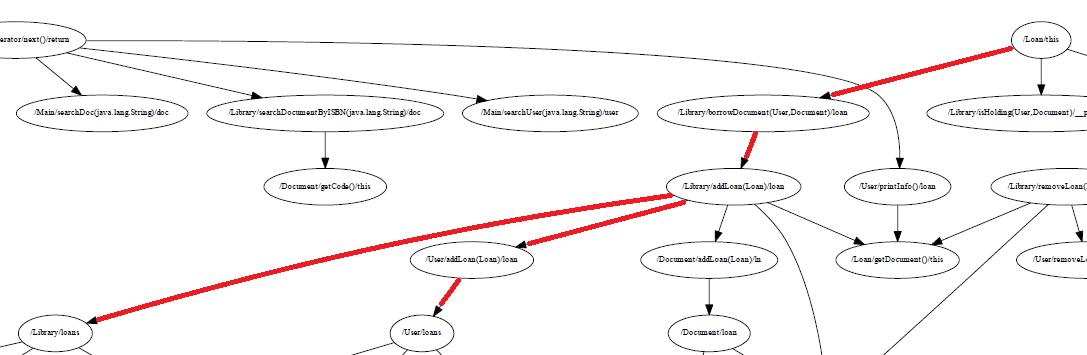
\includegraphics[angle=90,height=0.98\textheight]{loans}
				\caption{Reconstructed class diagram for edited version of eLib (with inner class and generics).}
				\label{fig:loans}
			\end{figure}

			When it comes to performance, we think our version is pretty slow. For eLib it takes about 1 minute to complete the rascal program, for which most of the time can be accounted to the extraction of associations using the OFG and the dependencies. There are some optimizations possible to the comprehensions we use there, but we decided to try and run our rascal program on a bigger project first to see if it really took too long.
			
		\subsection{Case study: CyberNeko HTML Parser}
			Now that the reconstruction tool chain has been tested on the smaller eLib project, we will look into the CyberNeko HTML Parser. CyberNeko HTML is also a java project so we import it into Eclipse and let the tool chain do the work. This didn't work instantly, since a lot of dependencies were missing, and the Java-extraction libraries from Rascal we are using require them to be present in order for them to work. After we manually import the dependencies in the Eclipse project, the tool chain returned the diagrams in Figures \ref{fig:neko1} and \ref{fig:neko2}. The diagrams visualize the architecture of CyberNeko HTML version 0.9.5 (December 2007), and version 1.9.14 (February 2010). \\

			\begin{figure}[h!]
				\centering
				\includegraphics[width=\textwidth]{nekohtml-095}
				\caption{Reconstructed class diagram CyberNeko HTML version 0.9.5.}
				\label{fig:neko1}
			\end{figure}
			
			\begin{figure}[h!]
				\centering
				\includegraphics[width=\textwidth]{nekohtml-1914}
				\caption{Reconstructed class diagram CyberNeko HTML version 1.9.14.}
				\label{fig:neko2}
			\end{figure}

			First we identify the similarities and differences between the two versions of the program, using the reconstructed class diagrams, and then we use this information to discuss how we think the system has evolved. We also look into the mailing lists and try to link changes there to the class diagrams. \\
			
			The easiest place to start is the upper right corner of the 0.9.5 version class diagram. There we see a small cluster of classes that is separated from the rest of the project. We see the ObjectFactory, with many static fields and methods and other classes it depends on. This part is identical in the 1.9.14, also in the upper right corner, but the Tester class is missing. We can explain this by the fact that there is a whole test directory besides the src directory, which is full of classes extending the Test Case class. As the project became bigger and bigger, there probably was a need for more extensive test suite than a class that can execute tests and compare output. \\

			The next part we consider is the HTMLConfiguration, with SAXParsers, DOM(fragment)Parser and ErrorReporter. This is identical in both of the diagrams and is probably part of the core of the system that is build first, and undergone little change throughout the lifetime of the project. HTMLConfiguration also has associations to both HTMLTagBalancer and HTMLScanner, which probably are also core features of CyberNeko HTML. The last association of HTMLConfiguration is to Script, which is one of the many specializations of DefaultFilter, just as Writer, ElementRemover, NamespaceBinder, Identity and Purifier. All of these are present in both versions. However the newer version has an extra specialization called Minimal, which is added later. \\

			The HTMLTagBalancer has associations with SynthesizedItem, HTMLAugmentations, Info and InfoStack and in the 1.9.14 version also is associated with a class named ElementEntry. ElementEntry is a small class that can be introduced for many reasons, such as a small added feature, unexpected behaviour that could be solved easily, etc. The HTMLScanner has the same associations in both versions, namely to ContentScanner, SpecialScanner, LocationItem, CurrentEntity, PlaybackInputStream, SynthesizedItem and HTMLAugmentations. A Scanner is an imporant part of a Parser and is therefore a core feature and most likely not changed a lot, outside of bugfixes.\\

			The last important classes from the 0.9.5 version we have not yet addressed are Element and HTMLElements. A lot of classses depend on them of have associations to them. They alse seem to be identical and part of the core of the system.\\

			A set of classes that is fully absent from the 0.9.5 version, but can be found in the 1.9.14 version is the XercesBridge and specializations. The Apache Xerces Project is responsible for the development and maintainance of XML parsers and related software components. Since CyberNeko HTML Parser heavily relies on the Xerces Java libraries, and these libraries also get updated with new versions, the developers of CyberNeko HTML must have come up with a convenient way to use the different versions of Xerces. The XercesBridge variants must be the result of this. \\
			
			We have also looked into the mailing lists associated to CyberNeko HTML, and in particular the user and developer mailing lists. What we found was that the user mailing list is not really usefull to find out about the evolution of the system. It is mostly about users asking wheter/how some feature is supported, or them doing a strange observation/bug report. You could probably find information about evolution if you scan through everything, but it is not so straightforward. However there are some mails about the releases of new versions, and they link to a webpage with changes per version. This is exactly what we need to find out how the project evolved. For example, here we can find that version 1.9.7 most likely started using the XercesBridge.\\

			The developer mailing list is far more useful when it comes to changes in the code. A big part of it consists of automated SVN messages, bug reports and request for supporting some feature. All of these messages come down to changes made in some particular part of the system. When we are looking into evolution, we are interested in changes, so this mailing list is perfect for getting information about evolution. However, in our case, it is really had to point out individual mails that are also visible in our class diagram, since they are mostly small changes that don't affect the architecture by a lot. Also the versions we reconstructed are pretty far separated in development, so there are many small changes in between. An example of information we can retrieve is for example that the \texttt{read()} of HTMLScanner is pretty important, and also buggy, since many bug reports and support requests are about this method. \\
			
			If we look at the visualization itself, we think we did a good job at reconstructing a fairly complete class diagram, supporting many features. It was a good idea to leave out some of the more complex features, since for big projects the diagram already seems messy. It might have been a good idea to merge bidirectional associations, since there are already many relations, so merging will reduce the amount a bit. We also see that some parts of the class diagram are in the same place and have the same structure in both diagrams, while for other parts the structure of the diagram changed, while it expresses the same thing. We need some kind of notion of hierarchy or grouping, as we stated before in the eLib example.//

			The performance of the tool chain was worse for the bigger project, as we already expected. The Rascal program takes about 15 minutes to extract all the information and generate the DOT-code. The problem is not so much the extraction of classes and data in the classes, but the relations between classes. We did not do any optimizations at this point, since we could already run the tool chain and get correct output. The bottleneck in this process was time, and waiting for 15 minutes was still pretty reasonable. GraphViz had no problems generating the diagram, once the DOT-code was obtained, and took only a couple of seconds.
			
	\section{Discussion of Tool Chain}
		Now that we have designed, implemented and tested the tool chain and also used it in a case study, we evaluate it based on our experiences with it. We have already pointed out a lot of advantages and disadvantages of our tool chain in the previous sections, so we will summarize them here. First we will look into the advantages of our approach:
		
		\begin{itemize}
			\item Modular Rascal program: We split the Rascal program into different modules, with each a distinct goal. The Extraction and Visualize module are even usable without the other. This made programming a lot easier, but it also had other advantages. Changes to the way of extraction did not affect the visualization and vice versa. If we would like to use a different ouput language of the Rascal program, so that we can use a different visualization tool, we can just write a new visualization module and still use the old Extraction module. We can also optimize the Extraction module, without affecting the Visualization.
			\item Leaving out complex structures. For bigger projects, the diagrams got more messy, and introducing more complex structures would only make it worse. A contradiction, in this case, would be the bidirectional associations, since they reduce the amount of relations a bit. Besides the clarity of diagrams, less complex things, means we have to do less calculations, which is advantageous for the performance of the Rascal program.
		\end{itemize}
		
		There are more apparent disadvantages to our tool chain, but most of them are related to the fact that our goal was to create a functional tool that reconstructed correct class diagrams, instead of creating a tool that was optimized computational- and visualization-wise.

		\begin{itemize}
			\item The performance of our Rascal program is a big disadvantage of the tool chain. This is related to two things: the separation of extraction and visualization, but also the inefficiency of the extraction part, with respect to use of comprehensions. Optimization of the Extraction code would already solve a big part of the problem.
			\item Diagrams can quickly become a bit messy, with many relations and little control over how classes are placed in the area. This was visible in the case study, where the structure of the project was the same in both versions, but the classes were ordered differently in the reconstructed diagrams. However, this is a limitation that can be solved by doing some extra computations to generate DOT-code that will declare more rules for the hierarchy and grouping of the classes in the generated diagram.
		\end{itemize}

		We think we did a fairly good job on creating a tool chain, that is not too hard to use, has a nice structure, and of which disadvantages can be addressed by further development.
	
	\section{Conclusions}
		We can conclude that architecture reconstruction is a nice way of getting insight in the evolution of a software project. All you need to do is reconstruct the architecture of different versions of a project and you have a convenient way of manually comparing the versions. Also using the right tools, it is not too hard to create a tool chain that does this reconstruction in a nice way. However, the more information you want to reconstruct in the diagram, and the nicer you want the diagram to be, the harder it is to get things right. Performance issues, and messy diagrams are the most apparant limitations to architecture reconstruction. We see this as a tradeoff: Having more complex features/visualization will require more computational power, but leaving out features will make room for other features to be more complex and computational demanding.

	\appendix
	\section{eLib Object Flow Graph}
	
		\begin{figure}[h!]
			\centering
			\includegraphics[angle=90,height=0.98\textheight]{OFGeLib}
			\caption{Object Flow Graph built for edited version of eLib (with inner class and generics).}
			\label{fig:ofgelib}
		\end{figure}

	\begin{thebibliography}{9}
		\bibitem{rascal}
			Rascal, Centrum Wiskunde \& Informatica , http://www.rascal-mpl.org/

		\bibitem{graphviz}
			GraphViz, Graph visualization software, http://www.graphviz.org/

		\bibitem{tonella}
			F. Tonella, A. Potrich. 
			Reverse Engineering of Object Oriented Code.
			Springer,
			2005.
			
		\bibitem{rascal-ofg}
			Rascal OFG, Davy Landman, https://github.com/cwi-swat/rascal-OFG
		
	\end{thebibliography}

\end{document}